\documentclass[a4paper,11pt,oneside]{article}
\usepackage[utf8]{inputenc}
\usepackage[a4paper,bindingoffset=0in, left=1.0in,right=1.0in,top=1.2in,bottom=1.2in]{geometry}
\usepackage{multicol}
\usepackage{graphicx} % Required for inserting images
\usepackage{fancyhdr}
\usepackage{mathrsfs}
\usepackage{amsmath}
\usepackage{amssymb}

\DeclareRobustCommand{\bbone}{\text{\usefont{U}{bbold}{m}{n}1}}
\DeclareMathOperator{\EX}{\mathbb{E}}% expected value

\usepackage{etoolbox}
\makeatletter
\patchcmd{\@maketitle}{\vskip 3em}{\vspace*{-3cm}}{}{}
\makeatother

\usepackage{titlesec}
\titleformat{\chapter}{\bfseries\LARGE}{\thechapter~}{1em}{}
\titlespacing{\chapter}{0in}{0in}{0.25in}

\usepackage[hyphens]{url}
\usepackage{hyperref}
\urlstyle{same} 
\hypersetup{colorlinks=true, linkcolor=black, filecolor=black, urlcolor=black, citecolor=blue}

\usepackage[british]{babel}
\usepackage{setspace}
\setstretch{1.5}
\usepackage{parskip}
\setlength{\parindent}{0pt}

\newcommand{\abbrlabel}[1]{\makebox[1in][l]{\textbf{#1}\ }}
\newenvironment{Abbreviations}{\begin{list}{}{\renewcommand{\makelabel}{\abbrlabel}}}{\end{list}}

\makeatletter
\renewcommand\@biblabel[1]{}
\renewenvironment{thebibliography}[1]
     {\section*{\refname}%
      \@mkboth{\MakeUppercase\refname}{\MakeUppercase\refname}%
      \list{}%
           {\leftmargin0pt
           \advance\leftmargin2em
           \setlength\itemindent{-2em}
            \@openbib@code
            \usecounter{enumiv}}%
      \sloppy
      \clubpenalty4000
      \@clubpenalty \clubpenalty
      \widowpenalty4000%
      \sfcode`\.\@m}
     {\def\@noitemerr
       {\@latex@warning{Empty `thebibliography' environment}}%
      \endlist}
\makeatother

\usepackage{cite}
\renewcommand\citeleft{}
\renewcommand\citeright{}

\pagestyle{plain}
\fancyhead[R]{Meier, Merki, and Thimóteo}
\fancyhead[C]{}
\fancyhead[L]{\rightmark}
\fancyfoot[L]{}
\fancyfoot[C]{\thepage}
\fancyfoot[R]{}



\begin{document}
%\vskip 5em
%\title{Currency risks for Swiss residents}
%\author{Thomas Meier \and Ivo Merki \and Mateus T}
%\date{December 19, 2023}
%\maketitle

\thispagestyle{empty}
\vspace{35px}
\vspace{35px}
\begin{center}
\large
\end{center}
\vspace{35px}
\begin{center}
\LARGE \textbf{Currency risks for Swiss residents}
\end{center}
\vspace{10px}
\begin{center}
\large \textit{03SMDFOEC008: Digital Tools for Finance} \\
\vspace{10px}
\large Dr. Igor Pozdeev
\end{center}
\vspace{35px}
\begin{center}
\large Department of Banking and Finance \\
\vspace{5px}
\large University of Zurich \\
\end{center}
\vspace{130px}
\vspace{10px}
\begin{table}[!htbp]
  \centering
  \begin{tabular}{ll}
  \large \href{mailto:thomaswilhelm.meier@uzh.ch}{Thomas Meier} \large \\ [3pt]
  \large \href{mailto:ivo.merki@uzh.ch}{Ivo Merki} \large  \\ [3pt]
  \large  \href{mailto:mateus.siqueirathimoteo@uzh.ch}{Mateus Thimóteo} \large  \\ [3pt]
  \end{tabular}
\end{table}
\vspace{50px}
\begin{center}
\large Submitted on December 19, 2023 \\
\end{center}







\newpage
\pagestyle{plain}
\setcounter{page}{1}
\pagenumbering{Roman}
\tableofcontents

\newpage
\pagestyle{plain}
\listoffigures
\addcontentsline{toc}{section}{List of Figures}

\begingroup
\vspace{4ex}
\let\clearpage\relax
\listoftables
\endgroup
\addcontentsline{toc}{section}{List of Tables}

\newpage
\pagestyle{plain}
\section*{Abbreviations}
\addcontentsline{toc}{section}{Abbreviations}
\begin{Abbreviations}
\item[DWT] Durbin-Watson-Test 
\item[CBOE] Chicago Board Options Exchange 
\item[CHF] Swiss franc
\item[EUR] Euro
\item[FRED] Federal Reserve Economic Data 
\item[OECD] Organisation for Economic Co-operation and Development
\item[SNB] Swiss National Bank
\item[UIP] Uncovered interest rate parity
\item[USD] US dollar
\item[VIX] CBOE Volatility Index
\end{Abbreviations}


\newpage
\pagestyle{fancy}
\setcounter{page}{1}
\pagenumbering{arabic}

\section{Introduction}\label{Introduction}
The COVID crisis in 2019 confirmed once more the safe haven currency status of the Swiss franc (CHF) based on the characteristic proposed by \cite{Habib and Stracca 2012}. While a safe haven currency status might be beneficial from a value storage perspective, it certainly presents challenges regarding other perspectives (see Figure \ref{fig:1}). The aim of this paper is to determine the riskiest currency to hold for a Swiss investor. It is based on the works of \cite{Grisse and Nitschka 2015}, \cite{Verdelhan 2010}, \cite{Backus and Foresi and Telmer 2001}, and \cite{Lustig and Roussanov and Verdelhan 2011}. The analysis consists of 9 CHF exchange rate pairs starting from April 2002 to November 2023 based on the framework of \cite{Grisse and Nitschka 2015} with one CHF-specific (\emph{AFX}) and one global risk factor (\emph{VIX}). Our results highlight the riskiness of AUD and CAD for Swiss investors. The paper is structured as follows. Section \ref{Theoretical background} briefly elaborates on the theoretical background. Section \ref{Data} discloses the data sources. Section \ref{Analysis} contains the analysis with the results. Section \ref{Conclusion} provides a conclusion.\par 

\begin{figure}[h]
    \centering
    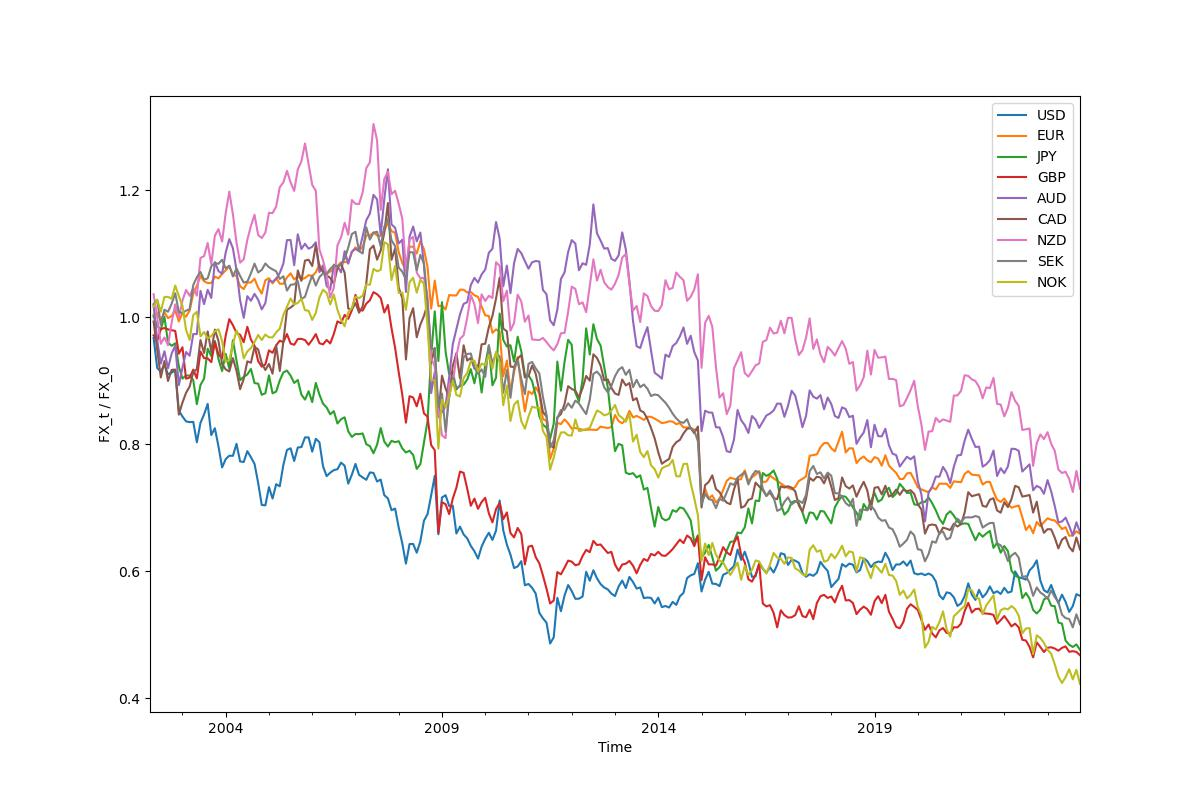
\includegraphics[width=\textwidth]{figures/ccy_perfs.jpg}
    \caption{Returns in different currencies}
    \label{fig:1}
\end{figure}


\newpage  
\section{Theoretical background}\label{Theoretical background}
This section aims to provide a very brief theoretical background to guide the reader through the analysis in the following section \ref{Analysis}.\par   

\subsection{Uncovered interest rate parity}\label{Uncovered interest rate parity}
The uncovered interest rate parity (UIP) states under the assumption of rational expectations and risk-neutrality an equality between the expected exchange rates change and the previous period`s interest rate differential between two countries (\cite{Grisse and Nitschka 2015}). This is expressed in the following formula \ref{1}.\par  

\begin{equation}\label{1}
\EX_{t}(\Delta s_{t+1}^k)= i_{t}^k-i_{t}^*
\end{equation}

where $\Delta s_{t+1}^k$ represents the change in the log spot exchange rates of the currencies, $i_{t}^k$ the foreign interest rate in country $k$, and $i_{t}^*$ the domestic interest rate.\par

Based on the findings of \cite{Akram and Rime and Sarno 2008} we consider as well as \cite{Grisse and Nitschka 2015} an approximate equality between monthly interest rate differentials and monthly forward discounts leading to the following formula \ref{2}.

\begin{equation}\label{2}
i_{t}^k-i_{t}^* \approx f_{t}^k-s_{t}^k
\end{equation}

where $f_{t}^k$ represents the log forward exchange rate. This results in the following model for the UIP regression:

\begin{equation}\label{3}
\Delta s_{t+1}^k=\alpha^k+\beta^k(f_{t}^k-s_{t}^k)+\epsilon_{t+1}^k
\end{equation}

where under the assumption that UIP holds, $\beta$ should be equal to one and $\alpha$ equal to zero. Due to limitations in the access of forward exchange rates, they were calculated with the following formula \ref{4}: 
\begin{equation}\label{4}
\mathcal{F}_{t,n}=S_{t}\frac{(1+i_{t,n}^*)^n}{(1+i_{t,n})^n}
\end{equation}

where $\mathcal{F}_{t,n}$ represents the forward exchange rate at time $t$ with maturity $n$, $S_{t}$ the spot exchange rate at time $t$, $i_{t,n}^*$ the domestic interest rate at time $t$ with maturity $n$, $i_{t,n}$ the foreign interest rate at time $t$ with maturity $n$. 

\subsection{Incorporation of currency risk factors}
The lack of empirical support for the holding of the UIP, as mentioned by \cite{Grisse and Nitschka 2015}, demands a solution. \cite{Verdelhan 2010} presents a feasible solution by incorporating currency risk factors into the UIP regression and therefore augmenting it. \cite{Grisse and Nitschka 2015} developed such an augmented model based on the work of \cite{Lustig and Roussanov and Verdelhan 2011} by incorporating an additional currency-specific risk factor and a global risk measurement on currency markets. While the currency-specific risk factor (\emph{AFX}) captures the average CHF exchange rate change across different CHF exchange rate pairs, the global risk measurement on currency markets is approximated by the \emph{VIX} due to its highly positive correlation (\cite{Grisse and Nitschka 2015}). By adding the previously mentioned additional risk factors to the regression it takes the following form:

\begin{equation}\label{5}
\Delta s_{t+1}^k=\alpha^k+\beta_{0}^k(f_{t}^k-s_{t}^k)+\beta_{1}^k AFX_{t+1}+\beta_{2}^k\Delta VIX_{t+1}+\epsilon_{t+1}^k
\end{equation}

where $AFX_{t+1}$ represents the arithmetic average of the CHF exchange rate changes (without currency $k$) and $\Delta VIX_{t+1}$ the log changes in the VIX.\par

\newpage
\section{Data}\label{Data}
The time span (April 2002 to November 2023) of the data is limited by the data series for Japan. This renders the bridge solution for the euro (EUR), as presented in \cite{Grisse and Nitschka 2015}, redundant. The exchange rates were retrieved as end-of-the-month US dollar (USD) cross-rates from the Federal Reserve Economic Data (FRED) and converted into end-of-the-month CHF exchange rates. The short-term interest rates were retrieved monthly as end of the month from the Organisation for Economic Co-operation and Development (OECD) database. The Chicago Board Options Exchange (CBOE) Volatility Index (VIX) was also retrieved monthly as end of the month from FRED.\par
 
%\newpage
\section{Analysis}\label{Analysis}
\subsection{Model}\label{Model}
\begin{equation}\label{5}
\Delta s_{t+1}^k=\alpha^k+\beta_{0}^k(f_{t}^k-s_{t}^k)+\beta_{1}^k AFX_{t+1}+\beta_{2}^k\Delta VIX_{t+1}+\epsilon_{t+1}^k
\end{equation}


\subsection{Results}\label{Results}
Our findings do not vastly deviate from those of \cite{Grisse and Nitschka 2015}. The constant $\alpha^k$ is almost zero and $\beta_{0}^k$ is as well as in \cite{Grisse and Nitschka 2015} statistically insignificant. Our analysis returned for the AUD a significantly negative AFX effect of -1.075 and a significantly negative log VIX change effect of -0.038. That probably makes the AUD the riskiest currency to hold for Swiss Investors. For the CAD our analysis returned a significantly negative AFX effect of -1.304 but an insignificantly negative log VIX change effect of -0.005. The Durbin-Watson-Test (DWT) is meant to check for auto-correlation. We did not find strong evidence for auto-correlation by running the DWT on the residuals. The DWT statistics return values between (1.92-2.13) coinciding with the values (1.70-2.24) returned by \cite{Grisse and Nitschka 2015}.\par

\newpage
\subsection{Robustness}
By including a control variable into our model representing the spreads between the 10-year Italian and 10-year German government bond yields we introduced a robustness check. This control variable aims to grasp euro area-related risks influencing the CHF exchange rates (\cite{Grisse and Nitschka 2015}). In line with the results reported by \cite{Grisse and Nitschka 2015} the control variable is in almost all regressions statistically insignificant with the exception of the USD in our regression. We also included another robustness check proposed by \cite{Brunnermeier and Nagel and Pedersen 2009} related to the TED spreads. The results for this robustness check are again in line with the results reported by \cite{Grisse and Nitschka 2015}.\par  


\section{Conclusion}\label{Conclusion}
A comparison of our results with the one of \cite{Grisse and Nitschka 2015} reveals vast similarities. We conclude that the AUD is probably the riskiest currency with respect to the significantly negative AFX and a significantly negative VIX. In second place comes the CAD with a significantly negative AFX, but an insignificantly negative VIX.\par 

\newpage
\pagestyle{plain}
\renewcommand{\refname}{Bibliography}
\addcontentsline{toc}{section}{Bibliography}
\begin{thebibliography}{99}

\bibitem[Akram, Rime, and Sarno (2008)]{Akram and Rime and Sarno 2008}\href{https://doi.org/10.1016/j.jinteco.2008.07.004}{Akram, Q. Farooq, Dagfinn Rime, and Lucio Sarno, 2008, Arbitrage in the foreign exchange market: Turning on the microscope, \textit{Journal of International Economics} 76, 237--253.}

\bibitem[Backus, Foresi, and Telmer (2001)]{Backus and Foresi and Telmer 2001}\href{https://doi.org/10.1111/0022-1082.00325}{Backus, David K., Silverio Foresi, and Chris I. Telmer, 2001, Affine Term Structure Models and the Forward Premium Anomaly, \textit{Journal of Finance} 56, 279--304.}

\bibitem[Brunnermeier, Nagel, and Pedersen (2009)]{Brunnermeier and Nagel and Pedersen 2009}\href{https://doi.org/10.1086/593088}{Brunnermeier, Markus K., Stefan Nagel, and Lasse H. Pedersen, 2009, Carry Trades and Currency Crashes, \textit{NBER Macroeconomics Annual} 23, 313--347.}

\bibitem[Grisse and Nitschka (2015)]{Grisse and Nitschka 2015}\href{https://doi.org/10.1016/j.jempfin.2015.03.006}{Grisse, Christian, and Thomas Nitschka, 2013, On financial risk and the safe haven characteristics of Swiss franc exchange rates, \textit{Journal of Empirical Finance} 32, 153--164.}

\bibitem[Habib and Stracca (2012)]{Habib and Stracca 2012}\href{https://doi.org/10.1016/j.jinteco.2011.12.005}{Habib, Maurizio M., and Livio Stracca, 2012, Getting beyond carry trade: What makes a safe haven currency?, \textit{Journal of International Economics} 87, 50--64.}

\bibitem[Lustig, Roussanov, and Verdelhan (2011)]{Lustig and Roussanov and Verdelhan 2011}\href{https://www.jstor.org/stable/41301998}{Lustig, Hanno, Nikolai Roussanov, and Adrien Verdelhan, 2011, Common Risk Factors in Currency Markets, pp.  in \textit{Review of Financial Studies} 24, 3731--3777.}

\bibitem[Verdelhan (2010)]{Verdelhan 2010}\href{https://doi.org/10.1111/j.1540-6261.2009.01525.x}{Verdelhan, Adrien, 2010, A Habit-Based Explanation of the Exchange Rate Risk Premium, \textit{Journal of Finance} 65, 123--146.}

\end{thebibliography}

\appendix
\newpage
\pagestyle{plain}
\setcounter{page}{1}
\pagenumbering{Roman}
\section*{Appendix}
\addcontentsline{toc}{section}{Appendix}

\begin{center}

% Table created by stargazer v.5.2.3 by Marek Hlavac, Social Policy Institute. E-mail: marek.hlavac at gmail.com
% Date and time: Sun, Dec 10, 2023 - 23:55:29
% Requires LaTeX packages: dcolumn 
\begin{table}[!htbp] \centering 
  \caption{} 
  \label{} 
\begin{tabular}{@{\extracolsep{5pt}}lD{.}{.}{-3} D{.}{.}{-3} D{.}{.}{-3} } 
\\[-1.8ex]\hline 
\hline \\[-1.8ex] 
 & \multicolumn{3}{c}{\textit{Dependent variable:}} \\ 
\cline{2-4} 
\\[-1.8ex] & \multicolumn{1}{c}{EUR\_} & \multicolumn{1}{c}{USD\_} & \multicolumn{1}{c}{JPY\_} \\ 
\\[-1.8ex] & \multicolumn{1}{c}{(1)} & \multicolumn{1}{c}{(2)} & \multicolumn{1}{c}{(3)}\\ 
\hline \\[-1.8ex] 
 F\_S\_EUR & -1.598 &  &  \\ 
  & (1.218) &  &  \\ 
  & & & \\ 
 F\_S\_USD &  & -0.728 &  \\ 
  &  & (1.403) &  \\ 
  & & & \\ 
 F\_S\_JPY &  &  & -2.176 \\ 
  &  &  & (2.495) \\ 
  & & & \\ 
 delta\_Log\_VIX & -0.002 & 0.040^{***} & 0.053^{***} \\ 
  & (0.004) & (0.007) & (0.008) \\ 
  & & & \\ 
 AFX\_EUR & -0.640^{***} &  &  \\ 
  & (0.042) &  &  \\ 
  & & & \\ 
 AFX\_USD &  & -0.906^{***} &  \\ 
  &  & (0.073) &  \\ 
  & & & \\ 
 AFX\_JPY &  &  & -0.557^{***} \\ 
  &  &  & (0.085) \\ 
  & & & \\ 
 Constant & -0.002 & -0.001 & -0.002 \\ 
  & (0.001) & (0.002) & (0.002) \\ 
  & & & \\ 
\hline \\[-1.8ex] 
Observations & \multicolumn{1}{c}{258} & \multicolumn{1}{c}{257} & \multicolumn{1}{c}{258} \\ 
R$^{2}$ & \multicolumn{1}{c}{0.496} & \multicolumn{1}{c}{0.392} & \multicolumn{1}{c}{0.215} \\ 
Adjusted R$^{2}$ & \multicolumn{1}{c}{0.490} & \multicolumn{1}{c}{0.385} & \multicolumn{1}{c}{0.205} \\ 
Residual Std. Error & \multicolumn{1}{c}{0.013 (df = 254)} & \multicolumn{1}{c}{0.022 (df = 253)} & \multicolumn{1}{c}{0.026 (df = 254)} \\ 
F Statistic & \multicolumn{1}{c}{83.310$^{***}$ (df = 3; 254)} & \multicolumn{1}{c}{54.480$^{***}$ (df = 3; 253)} & \multicolumn{1}{c}{23.147$^{***}$ (df = 3; 254)} \\ 
\hline 
\hline \\[-1.8ex] 
\textit{Note:}  & \multicolumn{3}{r}{$^{*}$p$<$0.1; $^{**}$p$<$0.05; $^{***}$p$<$0.01} \\ 
\end{tabular} 
\end{table} 

    \end{center}

\begin{center}

% Table created by stargazer v.5.2.3 by Marek Hlavac, Social Policy Institute. E-mail: marek.hlavac at gmail.com
% Date and time: Tue, Dec 19, 2023 - 21:05:04
% Requires LaTeX packages: dcolumn 
\begin{table}[!htbp] \centering 
  \caption{Regression Table GBP AUD CAD.} 
  \label{} 
\begin{tabular}{@{\extracolsep{5pt}}lD{.}{.}{-3} D{.}{.}{-3} D{.}{.}{-3} } 
\\[-1.8ex]\hline 
\hline \\[-1.8ex] 
 & \multicolumn{3}{c}{\textit{Dependent variable:}} \\ 
\cline{2-4} 
\\[-1.8ex] & \multicolumn{1}{c}{GBP\_} & \multicolumn{1}{c}{AUD\_} & \multicolumn{1}{c}{CAD\_} \\ 
\\[-1.8ex] & \multicolumn{1}{c}{(1)} & \multicolumn{1}{c}{(2)} & \multicolumn{1}{c}{(3)}\\ 
\hline \\[-1.8ex] 
 F\_S\_GBP & 0.902 &  &  \\ 
  & (1.167) &  &  \\ 
  & & & \\ 
 F\_S\_AUD &  & 0.345 &  \\ 
  &  & (1.138) &  \\ 
  & & & \\ 
 F\_S\_CAD &  &  & -0.067 \\ 
  &  &  & (1.687) \\ 
  & & & \\ 
 delta\_Log\_VIX & 0.005 & -0.038^{***} & -0.005 \\ 
  & (0.006) & (0.006) & (0.005) \\ 
  & & & \\ 
 AFX\_GBP & -0.962^{***} &  &  \\ 
  & (0.066) &  &  \\ 
  & & & \\ 
 AFX\_AUD &  & -1.075^{***} &  \\ 
  &  & (0.066) &  \\ 
  & & & \\ 
 AFX\_CAD &  &  & -1.304^{***} \\ 
  &  &  & (0.062) \\ 
  & & & \\ 
 Constant & 0.0002 & 0.001 & 0.001 \\ 
  & (0.002) & (0.003) & (0.003) \\ 
  & & & \\ 
\hline \\[-1.8ex] 
Observations & \multicolumn{1}{c}{258} & \multicolumn{1}{c}{258} & \multicolumn{1}{c}{258} \\ 
R$^{2}$ & \multicolumn{1}{c}{0.461} & \multicolumn{1}{c}{0.586} & \multicolumn{1}{c}{0.651} \\ 
Adjusted R$^{2}$ & \multicolumn{1}{c}{0.455} & \multicolumn{1}{c}{0.581} & \multicolumn{1}{c}{0.647} \\ 
Residual Std. Error (df = 254) & \multicolumn{1}{c}{0.020} & \multicolumn{1}{c}{0.020} & \multicolumn{1}{c}{0.018} \\ 
F Statistic (df = 3; 254) & \multicolumn{1}{c}{72.521$^{***}$} & \multicolumn{1}{c}{119.730$^{***}$} & \multicolumn{1}{c}{158.024$^{***}$} \\ 
\hline 
\hline \\[-1.8ex] 
\textit{Note:}  & \multicolumn{3}{r}{$^{*}$p$<$0.1; $^{**}$p$<$0.05; $^{***}$p$<$0.01} \\ 
\end{tabular} 
\end{table} 
%
\end{center}

\begin{center}

% Table created by stargazer v.5.2.3 by Marek Hlavac, Social Policy Institute. E-mail: marek.hlavac at gmail.com
% Date and time: Sun, Dec 10, 2023 - 23:17:51
% Requires LaTeX packages: dcolumn 
\begin{table}[!htbp] \centering 
  \caption{Regression Results 3} 
  \label{} 
\begin{tabular}{@{\extracolsep{5pt}}lD{.}{.}{-3} D{.}{.}{-3} D{.}{.}{-3} } 
\\[-1.8ex]\hline 
\hline \\[-1.8ex] 
 & \multicolumn{3}{c}{\textit{Dependent variable:}} \\ 
\cline{2-4} 
\\[-1.8ex] & \multicolumn{1}{c}{NZD\_} & \multicolumn{1}{c}{SEK\_} & \multicolumn{1}{c}{NOK\_} \\ 
\\[-1.8ex] & \multicolumn{1}{c}{(1)} & \multicolumn{1}{c}{(2)} & \multicolumn{1}{c}{(3)}\\ 
\hline \\[-1.8ex] 
 F\_S\_NZD & 1.395 &  &  \\ 
  & (1.149) &  &  \\ 
  & & & \\ 
 F\_S\_SEK &  & -0.319 &  \\ 
  &  & (1.530) &  \\ 
  & & & \\ 
 F\_S\_NOK &  &  & 0.710 \\ 
  &  &  & (1.479) \\ 
  & & & \\ 
 delta\_Log\_VIX & -0.038^{***} & -0.013^{**} & -0.025^{***} \\ 
  & (0.007) & (0.005) & (0.006) \\ 
  & & & \\ 
 AFX\_NZD & -0.862^{***} &  &  \\ 
  & (0.077) &  &  \\ 
  & & & \\ 
 AFX\_SEK &  & -0.795^{***} &  \\ 
  &  & (0.057) &  \\ 
  & & & \\ 
 AFX\_NOK &  &  & -0.921^{***} \\ 
  &  &  & (0.070) \\ 
  & & & \\ 
 Constant & 0.005 & -0.001 & -0.0004 \\ 
  & (0.004) & (0.002) & (0.003) \\ 
  & & & \\ 
\hline \\[-1.8ex] 
Observations & \multicolumn{1}{c}{258} & \multicolumn{1}{c}{258} & \multicolumn{1}{c}{258} \\ 
R$^{2}$ & \multicolumn{1}{c}{0.420} & \multicolumn{1}{c}{0.470} & \multicolumn{1}{c}{0.461} \\ 
Adjusted R$^{2}$ & \multicolumn{1}{c}{0.413} & \multicolumn{1}{c}{0.464} & \multicolumn{1}{c}{0.455} \\ 
Residual Std. Error (df = 254) & \multicolumn{1}{c}{0.023} & \multicolumn{1}{c}{0.017} & \multicolumn{1}{c}{0.021} \\ 
F Statistic (df = 3; 254) & \multicolumn{1}{c}{61.363$^{***}$} & \multicolumn{1}{c}{75.213$^{***}$} & \multicolumn{1}{c}{72.407$^{***}$} \\ 
\hline 
\hline \\[-1.8ex] 
\textit{Note:}  & \multicolumn{3}{r}{$^{*}$p$<$0.1; $^{**}$p$<$0.05; $^{***}$p$<$0.01} \\ 
\end{tabular} 
\end{table} 
%
\end{center}

%\includepdf[pages=1, scale=0.75,angle=90,pagecommand={\null\enlargethispage{\baselineskip}\vfill\captionof{figure}{Illustration of Value Proposition Canvas.}}]{VPC.pdf}


\end{document}



